% -*- coding: utf-8

\documentclass[slideopt,A4]{beamer}

\usetheme{default}

\useoutertheme{infolines}

\usepackage[]{fontspec}
\usepackage{fontenc}
\usepackage[type1]{libertine}
\renewcommand{\ttdefault}{cmtt}

\usepackage{lastpage}
\usepackage{mdframed}
\usepackage[usenames,dvipsnames,svgnames,table]{xcolor}


\usepackage{eurosym}
\usepackage{url}
\usepackage{anyfontsize}
\setmainfont{linuxbiolinumo}
\setsansfont{linuxbiolinumo}

\definecolor{fontmaincolor}{HTML}{000000}
\definecolor{bgcolor}{HTML}{FFFFFF}
\definecolor{bgshadecolor}{HTML}{DDDDDD}
\graphicspath{%
  {./Figures/}%
}
%\usepackage [T1] {inputenc}
%\usepackage [utf8] {inputenc}

\usepackage{tikz}
\usetikzlibrary{arrows,patterns,plotmarks,shapes,snakes,er,3d,automata,backgrounds,topaths,trees,petri,mindmap}
\usepackage{pgfplots}
\usepackage{pgfplotstable}

\usepackage{eso-pic}
\usepackage{monster2e}
\usepackage{tikz}
\usepackage{layout}
\usepackage{xcolor}
\usepackage{amsmath,amssymb,wasysym,bm}
\usepackage{fancybox}
\usepackage{graphicx}
\usepackage{subfigure}
\usepackage{multimedia}
\usepackage[absolute,showboxes,overlay]{textpos}
\TPshowboxesfalse
\textblockorigin{0mm}{0mm}

\usepackage{media9}
%\usepackage{movie15_dvipdfmx}
%\usepackage[dvipdfmx]{movie15_dvipdfmx}

\definecolor{rouge1}{RGB}{226,0,38}  % red P
\definecolor{orange1}{RGB}{243,154,38}  % orange P
\definecolor{jaune}{RGB}{254,205,27}  % jaune P
\definecolor{blanc}{RGB}{255,255,255} % blanc P

\definecolor{rouge2}{RGB}{230,68,57}  % red S
\definecolor{orange2}{RGB}{236,117,40}  % orange S
\definecolor{taupe}{RGB}{134,113,127} % taupe S
\definecolor{gris}{RGB}{91,94,111} % gris S
\definecolor{bleu1}{RGB}{38,109,131} % bleu S
\definecolor{bleu2}{RGB}{28,70,114} % bleu S
\definecolor{vert1}{RGB}{133,146,66} % vert S
\definecolor{vert2}{RGB}{157,193,7} % vert S

\definecolor{rouge3}{RGB}{255,200,130}  

\setbeamertemplate{navigation symbols}{}
\setbeamertemplate{blocks}[rounded][shadow=false]
\setbeamercolor{block title}{fg=white, bg=rouge1}
\setbeamercolor{block body}{fg=black, bg=rouge3}

\usepackage{tikz}
% tikz library (frise lncmi exemple)
\usetikzlibrary{calc,fit,shadows,arrows,positioning}
\usepackage{xcolor}
\xdefinecolor{fColor}{RGB}{0 81 145} % Light blue
\newcommand{\fColor}{fColor}

\newcommand{\topLegend}[2]{
  node [text centered,%
  shade,%
  top color=\fColor,%
  text justified,
  draw,%
  semithick,
  rounded corners=2pt,
  above,
  #1] {#2}}

\newcommand{\bottomLegend}[2]{
  node [text centered,%
  shade,%
  top color=\fColor,%
  text justified,
  draw,%
  semithick,
  rounded corners=2pt,
  below,
  #1] {#2}}

\newcommand{\topEvent}[3]{\draw[<-,very thick] (#1) coordinate (#2) (#2 |- xH axis) -- ++ (#3)}
\newcommand{\bottomEvent}[3]{\draw[<-,very thick] (#1) coordinate (#2) -- ++ (#3)}
\newcommand{\bottomGraphics}[2]{node[below,draw,inner sep=1pt,thin,rounded corners=1pt] {\includegraphics[#1]{#2}}}
\newcommand{\topGraphics}[2]{node[above,draw,inner sep=1pt,thin,rounded corners=1pt] {\includegraphics[#1]{#2}}}

% define trademark symbol
\def\registered{{\ooalign{\hfil\raise .00ex\hbox{\scriptsize R}\hfil\crcr\mathhexbox20D}}}

\renewcommand{\sfdefault}{lmss}
\sffamily

\setbeamersize{text margin left=1cm,text margin right=1cm}


\AtBeginSection[] {
  \begin{frame}<beamer>{Plan}
   \tableofcontents[sectionstyle=show/shaded,subsectionstyle=show/shaded/hide]
%    \tableofcontents[currentsection]
  \end{frame}
 }

\AtBeginSubsection[] {
  \begin{frame}<beamer>{Plan}
   \tableofcontents[sectionstyle=show/shaded,subsectionstyle=show/shaded/hide]
%    \tableofcontents[currentsection,currentssubection]
  \end{frame}
 }


\newcommand{\ds}{\displaystyle}
\newcommand{\dg}{^\circ}
\newcommand{\saut}{\vspace*{3mm}\\}
\newcommand{\RR}{\hbox{\bf I\hspace*{-1mm}R}}
%% Macros
\newcommand{\ddx}[1]{\ensuremath{\frac{\partial #1}{\partial x}}}
\newcommand{\ddy}[1]{\ensuremath{\frac{\partial #1}{\partial y}}}
\newcommand{\ddz}[1]{\ensuremath{\frac{\partial #1}{\partial z}}}
\newcommand{\dddxdx}[1]{\ensuremath{\frac{\partial^2 #1}{\partial x \partial x}}}
\newcommand{\dddxdy}[1]{\ensuremath{\frac{\partial^2 #1}{\partial x \partial y}}}
\newcommand{\dddydy}[1]{\ensuremath{\frac{\partial^2 #1}{\partial y \partial y}}}
\renewcommand{\div}{\operatorname{div}}
\renewcommand{\rot}{\operatorname{rot}}

\begin{document}


\setbeamertemplate{background canvas}[vertical shading][top=white,middle=white,bottom=white]

\setbeamertemplate{footline}{ \hspace{5em} \textcolor{white} {Les Mathématiques}\hspace{2em}\null \vspace*{3pt}}


\begin{frame}

\begin{textblock*}{15cm}(13mm,30mm)
{\textcolor{red} {
{\huge\bf Mathématiques appliquées: }\\[2mm]
{\huge\bf  des maths en lien avec la société}\\[2mm]
{\bf Modélisation Simulation et Optimisation}\\[8mm] }}
{\textcolor{black} {
%   	{\Large Philippe Helluy \& Christophe Prud'homme}\\[2mm]
	{\Large Université de Strasbourg}\\[2mm]
        \includegraphics[height=1.2cm]{LOGOS/logoCemosis}	\hspace*{40mm}	
        \includegraphics[height=1.2cm]{LOGOS/logoUDS}\\
      }}
\end{textblock*}

\end{frame}


%%%%%%%%%%%%%%%%%%%%%%%%%%%

\setbeamertemplate{background canvas}[vertical shading][top=blanc, middle=blanc,bottom=blanc]

\setbeamercolor{toto}{fg=white,bg=blue}

\setbeamertemplate{footline}
{
\begin{beamercolorbox}[wd=1\paperwidth,ht=15.5pt]{toto}
\hspace{-1.6mm}	
  \raisebox{1.2ex}
  {  \includegraphics[height=.6cm]{LOGOS/logoCemosis}}
  \raisebox{2.5ex}
  %{ P. Helluy \& C. Prud'homme (UNISTRA/CEMOSIS)  }
  {Cemosis, IRMA, UFR Math-Info}
\hspace{\fill}	
 % \raisebox{1.2ex}
%\hspace{\fill}	
%  \raisebox{2.5ex}
%  { \insertframenumber \hspace{1mm}  }
  \raisebox{2.5ex}
 {  }
  \raisebox{1ex}
{  \colorbox{white}{\includegraphics[height=.6cm]{LOGOS/logoUDS}}}
\end{beamercolorbox} 
}

%
%
%%%%%%%%%%%%%%%%%%%%%%%%%%%%%%%%%%%%%%

\begin{frame}{{\Large Plan}}
  \tableofcontents
  % Vous pouvez, si vous le souhaiter ajouter l'option [pausesections]
\end{frame}



%\begin{frame}
%Crypto: ajouter exemple de codage / décodage  eco spé maths TS\\[10mm]
%
%Simul: faire la discrétisation d'une équation de transport: 
%- on prend 2 boites, on écrit les quantités qui passent de l'une à l'autre en un pas de temps delta t
%- puis on en prend 3, etc...
%
%\end{frame}

%%%%%%%%%%%

\section{Mathématiques appliquées et métiers des maths}



\begin{frame}
\frametitle{Pour commencer...}

%\textcolor{black} 
%
%
%\begin{minipage}{70mm}
\begin{itemize}
\item {\large A quoi servent les mathématiques ?}
\item  {\large Y a-t-il des métiers après des études en mathématiques ?}
\end{itemize}
%\end{minipage}
%
\begin{center}
\includegraphics[width=0.20\linewidth]{maths2}$\quad$
\includegraphics[width=0.27\linewidth]{maths1}$\quad$
\includegraphics[width=0.24\linewidth]{einstein}
\end{center}

\begin{block}{Du coté de nos amis américains?}
  \begin{itemize}
  \item Un métier en pleine expansion: \\{\small\url{http://www.bls.gov/ooh/math/mathematicians.htm}}
  \item Best job en 2014:\\ {\small \url{http://www.careercast.com/jobs-rated/best-jobs-2014}}
  \end{itemize}
\end{block}
%
\end{frame}



%%%%%%%%%%%%%%%%%%%%%



\begin{frame}
\frametitle{Les mathématiques sont omniprésentes dans notre société}
%
%Les mathématiques sont omniprésentes dans notre société.
\begin{center}
\includegraphics[width=0.90\linewidth]{mix.png}
\end{center}

\end{frame}
%
%

\begin{frame}
\frametitle{Créer des images...}
%
\begin{center}
\includegraphics[width=0.40\linewidth]{LaraCroft.png}$\,$
\includegraphics[width=0.30\linewidth]{avatar}\\
\includegraphics[width=0.50\linewidth]{tintin}
\end{center}
%
\end{frame}
%
%
\begin{frame}
\frametitle{Créer des images...}
%
\begin{center}
\includegraphics[width=0.40\linewidth]{tete.png}$\quad$
\includegraphics[width=0.40\linewidth]{tete2.png}
\end{center}
%
\end{frame}
%


%
\begin{frame}
\frametitle{Compresser les images et les sons: MP3, MP4, jpeg, mov...}
%
\begin{center}
\begin{tabular}{cc}
\textcolor{red}{Image originale} & \textcolor{red}{Image compressée} \\
\includegraphics[width=0.40\linewidth]{lana-original.png} &
\includegraphics[width=0.40\linewidth]{lana-compresse.png}
\end{tabular}
\end{center}
%
\pause
%
\begin{center}
~\\[-10mm]
\includegraphics[width=0.4\linewidth]{ipod.jpg}
\end{center}
%
\end{frame}
%

%
\begin{frame}
\frametitle{Compresser les images et les sons: MP3, MP4, jpeg, mov...}
%
\includegraphics[width=0.3\linewidth]{fourier} $\qquad$
\includegraphics[width=0.5\linewidth, angle=-1.5]{fourier4} \\[5mm]
\centerline{\includegraphics[width=0.6\linewidth]{fourier2}}
%
\end{frame}
%

%
\begin{frame}
\frametitle{Imagerie médicale...}
\small
%
%
\begin{block}{Principe}
On soumet le corps à un signal (magnétique, électrique, acoustique, ...), et en fonction de la réponse obtenue, on reconstruit  une image de la zone observée (problème inverse).
\end{block}
%
\centerline{\includegraphics[width=0.7\linewidth]{imagerie-medicale.png}}
%
\end{frame}
%

%

\begin{frame}
  \frametitle{Santé}
  
  \begin{block}{}
    Comprendre les mécanismes physiologiques et
    pathologiques(anévrismes, anémie, atherosclérose, maladies
    neurodégénératives: Alzheimer...),
    proposer des outils de diagnostics peu chers et fiables
  \end{block}

\includegraphics[width=0.3\linewidth]{Figures/MesoChallengePressure2.png}$\;$
\includegraphics[width=0.3\linewidth]{Figures/sickleCellDisease.jpg}$\;$
\includegraphics[width=0.3\linewidth]{Figures/atherosclerosisDisease.jpg}\\
\centerline{\includegraphics[width=0.6\linewidth]{Figures/Eye2Brain_connections.pdf}}
  
\end{frame}

%
\begin{frame}
\frametitle{Statistiques...}
%
%
\includegraphics[width=0.3\linewidth]{medicaments.jpg}$\;$
\includegraphics[width=0.3\linewidth]{banque}$\;$
\includegraphics[width=0.3\linewidth]{assurance}
%
\end{frame}
%


%
\begin{frame}
\frametitle{Crypter...}
%
% 
\begin{minipage}{5cm}
~\\[-50mm]
\includegraphics[width=0.75\linewidth]{carte-bleue.jpg}\\
\includegraphics[width=0.95\linewidth]{paypal.jpg}
\end{minipage}
\includegraphics[width=0.5\linewidth]{reseau}
%
\end{frame}
%



%
\begin{frame}
\frametitle{Modéliser...}
%
%
\begin{minipage}{35mm}
\includegraphics[width=0.99\linewidth]{edf.png}
\end{minipage}$\;$
\begin{minipage}{70mm}
\includegraphics[width=0.99\linewidth]{edf2.png}\\[10mm]
\centerline{\alert{EDF}}
\end{minipage}
%
\end{frame}
%

%
\begin{frame}
\frametitle{Modéliser...}
%
Stockage de déchets radioactifs $\rightarrow$ Modélisation des écoulements en milieux poreux autour du site\\
\centerline{\includegraphics[width=0.8\linewidth]{stockage.png}}
%
\end{frame}
%

%
\begin{frame}
\frametitle{Modéliser...}
%
Contrôle non destructif
%
\centerline{\includegraphics[width=0.75\linewidth]{controle-nondestructif.png}}
%
\end{frame}
%


%
\begin{frame}
\frametitle{Modéliser...}
%
Fusion nucléaire contrôlée : plasma confiné dans la chambre magnétique (ITER)
%
\centerline{\includegraphics[width=0.8\linewidth]{iter.png}}
%
\end{frame}
%




%
\begin{frame}
\frametitle{Modéliser...}
%
% 

\includegraphics[width=0.4\linewidth]{voiture.png}$\qquad$
\includegraphics[width=0.5\linewidth]{pneu.png}\\[3mm]
\centerline{\includegraphics[width=0.5\linewidth]{avion}}
%
\end{frame}
%

%
\begin{frame}
\frametitle{Modéliser...}
%
% 
\centerline{
\includegraphics[width=0.2\linewidth]{chaise.png}$\qquad$
\includegraphics[width=0.2\linewidth]{coca}$\qquad$
\includegraphics[width=0.2\linewidth]{lessive} }
%
\end{frame}
%

\begin{frame}
  \frametitle{Calculer...}
  TGCC Curie: 10080 eight-core processors, Intel® Xeon® Next
  Generation, un total de 80640 cores.
  \centerline{\includegraphics[width=0.5\linewidth]{Figures/tgcc_curie.jpeg}}
  \centerline{Puissance énergie : 7.5 Mw ($\approx$ ville de 40 000 habitants)}\\
  \centerline{Puissance calcul: 200 Tflops, $200.10^{12}$ floating point
    operations per second}\\
  \begin{center}
    Ce type d’ordinateur est plus difficile à programmer qu’un PC (surtout si l’on veut que le calcul soit efficace !!).
  \end{center}
    \centerline{\alert{−→ informatique, algorithmique, optimisation...}}
\end{frame}

%
\begin{frame}
\frametitle{Il y a des dizaines de "métiers des maths" {\small (pas seulement prof !) }}
%
\begin{center}
\includegraphics[width=0.4\linewidth]{onisep.pdf}
\end{center}
%
\centerline{\htmladdnormallink{Quels Métiers pour les matheux? (ONISEP!)}{http://www.onisep.fr/Toute-l-actualite-nationale/Decouvrir-les-metiers/Decembre-2014/Quels-metiers-pour-les-matheux}}
%
\end{frame}

\section{Un peu d'Histoire}

\begin{frame}
  \frametitle{Encore un peu d'histoire}

  \begin{block}{Newton, Isaac (1642-1727) }
    \begin{columns}[c]
      \begin{column}{.3\textwidth}
        \includegraphics[height=.25\textheight]{figures/jpegs/prudhomme/Newton}
      \end{column}
      \begin{column}{.55\textwidth}
        All in nature reduces to differential equations
      \end{column}
    \end{columns}

  \end{block}

  \begin{block}{Planck, Max (1858-1947)}
    \begin{columns}[c]
      \begin{column}{.3\textwidth}
        \includegraphics[height=.25\textheight]{figures/jpegs/prudhomme/Planck}
      \end{column}
      \begin{column}{.55\textwidth}
        ...Present day physics, as far as it is theoritically organized,
        is completely governed by a system of space-time differential
        equations.
      \end{column}
    \end{columns}
  \end{block}
 \end{frame}

\begin{frame}
  \frametitle{Pourquoi s'intéresser aux EDPs?}

  \begin{block}{}
    \begin{itemize}
    \item Argent:
      \begin{itemize}
      \item Modifier la géométrie d'un véhicule pour réduire significativement la trainée (voiture, avion,...)
      \item modélisation des instruments financiers (derivatives)
      \end{itemize}
    \item Artistique:
      \begin{itemize}
      \item Acoustique
      \end{itemize}
    \item Curiosité Scientifique:
      \begin{itemize}
      \item Modéliser des phénomènes physiques encore mal compris  (turbulence)
      \item Modèles astrophysique, modèle solaire
      \end{itemize}
    \item Application en Ingénierie
      \begin{itemize}
      \item Modélisation des structures
      \item Electromagnétisme , acoustique, dynamique des fluides
      \end{itemize}
  \end{itemize}

  \end{block}

\end{frame}

\begin{frame}
  \frametitle{Pourquoi s'intéresser aux EDPs? }

  \begin{block}{}
      \begin{itemize}
    \item Environnement:
      \begin{itemize}
      \item Modélisation de l'impact des gaz à effet de serre
      \item Modélisation du temps pour éviter les dommages et prédire la performance des récoltes
      \item Prédire les tremblements de terre, les éruptions volcaniques, les tsunamis (Aussi section ``Argent'' ?)
      \end{itemize}
    \item Défense:
      \begin{itemize}
      \item Design de matériau et profiles pour des avions furtifs
      \item La bonne gestion du stock d'armes nucléaires
      \end{itemize}

  \end{itemize}

  \end{block}

  \begin{alertblock}{Discussion}
    Que vous vient il encore à l'esprit? Quel rang donneriez vous aux thèmes précédents ? Quel financement pour chacun ?
  \end{alertblock}
\end{frame}

\begin{frame}
  \frametitle{Les ingrédients d'une EDP}
  \begin{block}{Forme Abstraite d'une EDP}
    trouver $u = u(x,y,z,t)$ telle que
    \begin{equation}
      \label{eq:1}
      \frac{\partial u }{\partial t} = F( x, y, z, u, \ddx{u}, \ddy{u}, \ddz{u}, \dddxdx{u}, ... )
    \end{equation}
    \begin{itemize}
    \item $u$ Champs scalaire ou vectoriel (e.g. température, vitesse, pression,...)
    \item \ddx{u}, \dddxdx{u} dérivées partielles, mais aussi $\nabla u, \nabla \cdot u, \nabla \times u$
    \item $F$ est donnée par la physique ou la mécanique et fait l'objet
      d'\alert{aller-retours entre expérimentation, modélisation et
        simulation}
    \item $=$ Calcul
    \end{itemize}


  \end{block}
\end{frame}

\begin{frame}
  \frametitle{Cycle: Expérimentations, Modélisation, Simulation}

  \note[item]{On explique ici : \alert{aller-retours entre
      expérimentation, modélisation et simulation}}

  \tikzstyle{root concept}+=[concept color=white!80]
  \tikzstyle{level 1 concept}+=[concept color=red!80, sibling angle=120]
  \tikzstyle{every annotation}=[fill=black!50,opacity=0.5,text=white,scale=.7]
  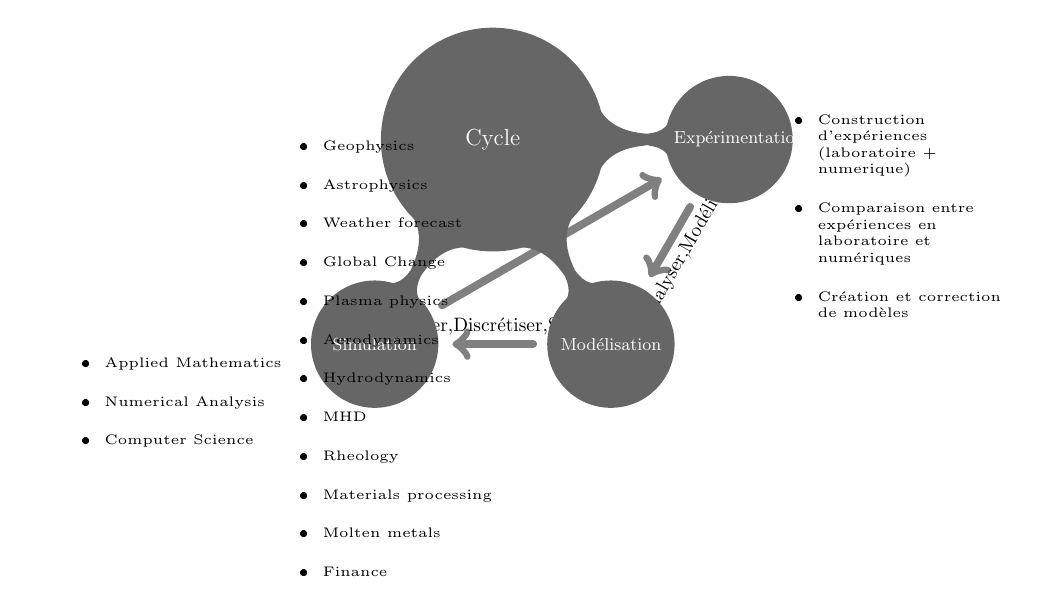
\begin{tikzpicture}[->]
    \path[mindmap,concept color=black!60,text=white]
    node[concept,scale=.7] {Cycle}
    %node[concept,scale=.7] {Scientific Computing}
    [clockwise from=0]
    % child[concept,scale=.6] { node[concept,scale=.7] (phys) {Physics Mechanics Biology Processing} }
    child[concept,scale=.6] { node[concept,scale=.7] (exp) {Exp\'erimentation} }
    child[concept,scale=.6] { node[concept,scale=.7] (mod) {Mod\'elisation} }
    child[concept,scale=.6] { node[concept,scale=.7] (sim) {Simulation} };

    \node [annotation,left] at (mod.west)
    {
      \begin{itemize}
      \item Geophysics
      \item Astrophysics
      \item Weather forecast
      \item Global Change
      \item Plasma physics
      \item Aerodynamics
      \item Hydrodynamics
      \item MHD
      \item Rheology
      \item Materials processing
      \item Molten metals
      \item Finance
      \end{itemize}
    };
    \node [annotation,left] at (sim.south west)
    {
      \begin{itemize}
      \item Applied Mathematics
      \item Numerical Analysis
      \item Computer Science
      \end{itemize}
    };
    \node [annotation,right] at (exp.south)
    {
      \begin{itemize}
      \item Construction d'expériences (laboratoire + numerique)
      \item Comparaison entre expériences en laboratoire et numériques
      \item Création et correction de modèles
      \end{itemize}
    };

    \begin{pgfonlayer}{background}
      \draw [concept connection]
      (exp) edge node[below,sloped,scale=.7]{Analyser,Modéliser} (mod)
      (mod) edge node[above,sloped,scale=.7]{Analyser,Discrétiser,Simuler} (sim)
      (sim) edge node[above,sloped,scale=.7]{Valider} (exp);
    \end{pgfonlayer}

  \end{tikzpicture}
\end{frame}

\begin{frame}
  \frametitle{Cycle de la simulation numérique}

  \tikzstyle{root concept}+=[concept color=white!80]
  \tikzstyle{level 1 concept}+=[concept color=red!80, sibling angle=72]
  \tikzstyle{every annotation}=[fill=black!50,opacity=0.5,text=white,scale=.7]
  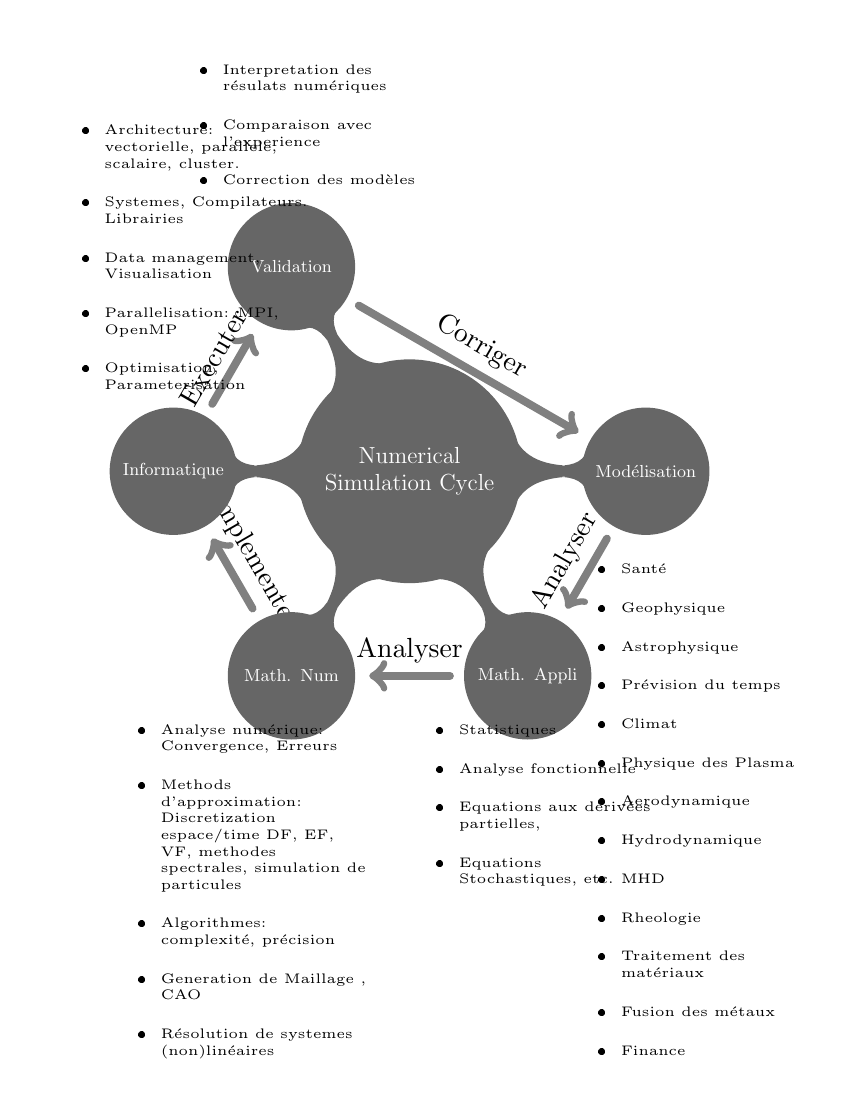
\begin{tikzpicture}[->]
     \path[mindmap,concept color=black!60,text=white]
     node[concept,scale=.7] {Numerical Simulation Cycle}
     %node[concept,scale=.7] {Scientific Computing}
     [clockwise from=0]
     %child[concept,scale=.6] { node[concept,scale=.7] (phys) {Physics Mechanics Biology Processing} }
     child[concept,scale=.6] { node[concept,scale=.7] (phys) {Modélisation} }
     child[concept,scale=.6] { node[concept,scale=.7] (am) {Math. Appli} }
     child[concept,scale=.6] { node[concept,scale=.7] (nm) {Math. Num} }
     child[concept,scale=.6] { node[concept,scale=.7] (cs) {Informatique} }
     child[concept,scale=.6] { node[concept,scale=.7] (va) {Validation} }
     ;
     \node [annotation,below] at (phys.south east)
     {
       \begin{itemize}
       \item Santé
       \item Geophysique
       \item Astrophysique
       \item Prévision du temps
       \item Climat
       \item Physique des Plasma
       \item Aerodynamique
       \item Hydrodynamique
       \item MHD
       \item Rheologie
       \item Traitement des matériaux
       \item Fusion des métaux
       \item Finance
       \end{itemize}
     };
     \node [annotation,below] at (am.mid)
     {
       \begin{itemize}
       \item Statistiques
       \item Analyse fonctionnelle
       \item Equations aux dérivées partielles,
       \item Equations Stochastiques, etc.
       \end{itemize}
     };
     \node [annotation,below] at (nm.west)
    {
      \begin{itemize}
      \item Analyse numérique:
        Convergence, Erreurs
      \item Methods d'approximation:
        Discretization espace/time
        DF, EF, VF,  methodes
        spectrales, simulation de particules
      \item Algorithmes: complexité, précision
      \item Generation de Maillage , CAO
      \item Résolution de systemes (non)linéaires
      \end{itemize}
    };
    \node [annotation,above] at (cs.north)
    {
    \begin{itemize}
    \item Architecture: vectorielle, parallele,  scalaire, cluster.
    \item Systemes, Compilateurs. Librairies
      \item Data management, Visualisation
      \item Parallelisation: MPI, OpenMP
      \item Optimisation, Parameterisation
      \end{itemize}
    };
    \node [annotation,above] at (va.north)
    {
      \begin{itemize}
      \item Interpretation des résulats numériques
      \item Comparaison avec l'experience

      \item \alert{Correction des modèles}
      \end{itemize}
    }
    ;

    \begin{pgfonlayer}{background}
      \draw [concept connection]
      (phys) edge node[above,sloped]{Analyser} (am)
      (am) edge node[above,sloped]{Analyser} (nm)
      (nm) edge node[above,sloped]{Implementer} (cs)
      (cs) edge node[above,sloped]{Executer} (va)
      (va) edge node[above,sloped]{Corriger} (phys);
     \end{pgfonlayer}

\end{tikzpicture}
\end{frame}




\section{Quelques exemples}
\label{sec:quelques-exemples}


%%% Local Variables: 
%%% mode: latex
%%% TeX-master: "slides-math-formations-metiers"
%%% End: 

\subsection{Santé}
\begin{frame}
  
\end{frame}

%%% Local Variables: 
%%% mode: latex
%%% TeX-master: "slides-math-formations-metiers"
%%% End: 

\subsection{Champs Magnétiques Intenses}
\begin{frame}{Laboratoire National des Champs Magn\'etiques Intenses}
  \begin{columns}[c]
    \begin{column}{0.5\textwidth}
      \begin{alertblock}{ \begin{small} Grand équipement francais (CNRS) \end{small}}
        \begin{small}
          \begin{itemize}
          \item Champs magnétiques intenses : à partir de 24 T.
          \end{itemize}
        \end{small}
      \end{alertblock}
    \end{column}
    \begin{column}{0.5\textwidth}
      \begin{alertblock}{}
        \begin{small}
          \begin{itemize}
          \item À Grenoble, champ continu max : 36 T
            (objectif 40-45T).
          \end{itemize}
        \end{small}
      \end{alertblock}
    \end{column}
  \end{columns}

  \vspace*{-0.4cm}
  \begin{tikzpicture}[scale=0.42][%
    >=latex,%
    font=\fontfamily{phv}\fontsize{7}{8}\selectfont,
    legend/.style={%
      draw,
      rounded corners=2pt,
      shade}]

    % frise 
    \draw[rounded corners,shade,left color=fColor!40,right color=fColor!5] (-14,0) -- ++ (26,0) -- ++ (1,1.5) -- ++(-1,1.5) -- ++ (-26,0) -- cycle;
    % axe bas
    \path (-10,0) -- (10,0) coordinate (xL axis);
    % axe haut
    \path[yshift=+3cm]         (-10,0) -- (10,0) coordinate (xH axis);
    % rupture
    \path[] (+0.5,-0.25) rectangle ++(8mm,3.5) node [midway,rotate=90,minimum width=3.5cm,shade,sharp corners,inner sep=1pt] (r1) {36 tesla};
    \draw[densely dotted] (r1.south east) -- (r1.south west) (r1.north east) -- (r1.north west);
    \draw[thick] (1.5,0) -- (1.5,-30mm) \bottomGraphics{width=3cm}{Figures/cmi/polyhelix.jpg};
    \draw[] (0,0) coordinate (an0) -- (an0 |- xH axis) -- ++ (0,2.5mm) node [above] {$10^0$};


    % scope 1
    \begin{scope}[xshift=3cm,xscale={14cm/400cm}]
      % graduation
      \draw[] (0,0)   coordinate (an0) -- (an0 |- xH axis) -- ++ (0,2.5mm) node [above] {$10^{+2}$};
      \draw[] (100,0) coordinate (an100) -- (an100 |- xH axis) -- ++ (0,2.5mm) node [above] {$10^{+3}$};
      \draw[] (200,0) coordinate (an200) -- (an200 |- xH axis) -- ++ (0,2.5mm) node [above] {$10^{+9}$};

      % evennement
      \topEvent{0,0}{an1617}{0,28mm} \topLegend{text width=4.5cm,name=r}{100 t :\\Pulsed magnetic field (ND) (USA)};
      \bottomEvent{127,0}{an1727}{0,-10mm} \bottomLegend{text width=4.5cm}{2800 t :\\Pulsed magnetic field (D) (Russia)};
      \topEvent{200,0}{an1617}{0,12mm} \topLegend{text width=2cm}{100 Mt to 100 Gt :\\Magnetar};
    \end{scope}

    % scope 2
    \begin{scope}[xshift=0cm,xscale={0.7cm/30cm}]
      % graduation
      \draw[] (-100,0) coordinate (anM1000) -- (anM1000 |- xH axis) -- ++ (0,2.5mm) node [above,fill=white] {$10^{-1}$};
      \draw[] (-200,0) coordinate (anM2000) -- (anM2000 |- xH axis) -- ++ (0,2.5mm) node [above,fill=white] {$10^{-2}$};
      \draw[] (-300,0) coordinate (anM3000) -- (anM3000 |- xH axis) -- ++ (0,2.5mm) node [above,fill=white] {$10^{-5}$};
      \draw[] (-500,0) coordinate (anM4000) -- (anM4000 |- xH axis) -- ++ (0,2.5mm) node [above,fill=white] {$10^{-12}$};
      % evennement

      \bottomEvent{6,0}{anM30}{0,-30mm} \bottomLegend{text width=2.5cm}{$1.5$ to 3 t : \\medical MRI systems};

      \topEvent{-173,0}{anM1730}{0,12mm} \topLegend{text width=2.5cm}{0.5 mt :\\limit for pacemakers};
      \bottomEvent{-300,0}{anM1730}{0,-10mm} \bottomLegend{text width=3cm}{31 to 100 $\mu$t :\\Earth's magnetic field};
      \topEvent{-500,0}{anM3730}{0,12mm} \topLegend{text width=2cm}{$10^{-12}$ t :\\Human brain};
    \end{scope}
  \end{tikzpicture}
\end{frame}

\begin{frame}{Laboratoire National des Champs Magn\'etiques Intenses}

   Installation champs pulsés à TOULOUSE : 14 MJ, 24 kV, 1 GW, 80 Tesla
   \vskip-0.3cm
   \begin{figure}[H]
    \centering
    \includegraphics[scale=0.3]{Figures/cmi/powersupply_pulsed.png}
   \end{figure}

   Installation champs continus à GRENOBLE: 24 MW,  36 Tesla
   \vskip-0.3cm

 \begin{columns}[c]
  \begin{column}{8cm}
   \begin{figure}[H]
    \centering
    \includegraphics[scale=0.2]{Figures/cmi/powersupply.png}
   \end{figure}
  \end{column}

  \begin{column}{5cm}
   \begin{figure}[H]
    \centering
    \includegraphics[scale=0.4]{Figures/cmi/magnet.png}
   \end{figure}
  \end{column}
 \end{columns}
\end{frame}

% \begin{frame}{Champs magnétiques intenses : domaines d'application}
%   \begin{columns}
%     \begin{column}{0.55\textwidth}
%       \begin{small}
%         \begin{itemize}
%         \item Supraconductivité appliquée ;
%         \item Science du magnétisme ;
%         \item (Bio-)Chimie ;
%         \end{itemize}
%       \end{small}

%     \end{column}

%     \begin{column}{0.55\textwidth}
%       \begin{small}
%         \begin{itemize}
%         \item Physique du solide (Résonance Magnétique Nucléaire) ;
%         \item Lévitation magnétique ;
%         \item ...
%         \end{itemize}
%       \end{small}

%     \end{column}
%   \end{columns}

%   \begin{figure}[H]
%     \includegraphics[scale=0.5]{Figures/cmi/research.png}
%   \end{figure}
% \end{frame}

\begin{frame}{Champs Magnétiques Intenses : à quoi ça sert ?}
    \begin{columns}[c]
      \begin{column}{0.78\textwidth}
        \begin{block}{Reproduire les conditions de zero-gravité}
          Moteur d'ariane 6 (SNECMA) : 
          \begin{itemize}
          \item Comment se comporte l'hydrogène liquide (carburant) en apesanteur ?
            \begin{itemize}
            \item Données d'entrée pour le design du moteur
            \item Moins coûteux qu'une expérience en conditions "réelles"
              \begin{itemize}
              \item heure de champ intense ($\approx$ 1000 \euro)
              \item vol parabolique ($\approx$ 100.000 \euro)
              \item vol dans l'espace ($\approx$ 10.000.000 \euro)
              \end{itemize}
            \end{itemize}
          \end{itemize}
          \vspace*{-0.4cm}
          \begin{columns}[c]
            \begin{column}{0.5\textwidth}
              \begin{figure}[H]
                \centering
                \includegraphics[scale=0.1]{Figures/cmi/levitation_1.png}
              \end{figure}
            \end{column}
            \begin{column}{0.5\textwidth}
              \begin{figure}[H]
                \centering
                \includegraphics[scale=0.12]{Figures/cmi/levitation_2.png}
              \end{figure}
            \end{column}
          \end{columns}
        \end{block}
      \end{column}
      \begin{column}{0.25\textwidth}
        \begin{figure}[H]
          \centering
          \includegraphics[scale=0.12]{Figures/cmi/ariane6_2.jpg}
        \end{figure}
      \end{column}
    \end{columns}
\end{frame}

\begin{frame}{Champs Magnétiques Intenses : à quoi ça sert ?}

  \begin{block}{Etudier les propriétés magnétiques}
    Optimisation de la capacité des disques durs
    \begin{itemize}
    \item Capacité dépend des propriétés magnétiques
      \begin{itemize}
      \item Revetement des disques : oxyde de fer (magnétique)
      \item Ecriture d'un bit : envoi d'une charge magnétique
      \item Lecture d'un bit : mesure de son champ magnétique
      \end{itemize}
    \end{itemize}
    \vspace*{-0.3cm}
    \begin{figure}[H]
      \centering
      \includegraphics[scale=0.2]{Figures/cmi/disk.png}
    \end{figure}

    Compréhension/Optimisation des propriétés magnétiques :
    \vspace*{-0.2cm}
    \begin{center}
      Mega-octets (Mo) $~\longrightarrow~$ Giga-octets (Go) $~\longrightarrow~$ Tera-octets (To)
    \end{center}
  \end{block}

\end{frame}

\begin{frame}{Electro-Aimants : à quoi servent les modèles ?}
  \begin{block}{Avant la mise en service : Développement des aimants}
    \begin{small}
      \begin{itemize}
      \item Augmenter l'intensité du champ magnétique
      \item Améliorer sa qualité (homogénéité)
      \end{itemize}
    \end{small}
    \vspace*{-0.5cm}
    \begin{center} \textbf{Optimisation $\Rightarrow$ Modélisation (fine) des electro-aimants} \end{center}
    \vspace*{-0.3cm}
    \begin{small}
      \begin{itemize}
      \item Permet de couvrir une large gamme de paramètres
        \begin{itemize}
        \item Envisager autant de cas que l'on veut pour trouver le design "optimal"
        \end{itemize}
      \item Possibilité de prévoir/anticiper les scénarios "catastrophes"
        \begin{itemize}
        \item Et éviter la casse (très couteuse!)
        \end{itemize}
      \end{itemize}
    \end{small}
  \end{block}
\end{frame}

\begin{frame}{Electro-Aimants : à quoi servent les modèles ?}
  \begin{block}{Après la mise en service : Lors d'un incident}
    \begin{small}
      \begin{itemize}
      \item Identifier/Comprendre la cause de l'incident
        \begin{itemize}
        \item Temperature trop elevée ? Problème mécanique ?
        \end{itemize}
      \end{itemize}
      \begin{figure}[H]
        \centering
        \includegraphics[scale=0.15]{Figures/cmi/loupe.jpg}
      \end{figure}
    \end{small}
    \vspace*{-0.4cm}
    \begin{center} \textbf{Analyse $\Rightarrow$ Reproduire l'incident par la simulation} \end{center}
    \vspace*{-0.4cm}
    \begin{small}
      \begin{itemize}
      \item Trouver une solution pour éviter que l'incident se reproduise : optimisation avant (re-) mise en service
      \end{itemize}
    \end{small}
  \end{block}
\end{frame}

%\subsection{Magnet study requires multi-physics modeling}
\begin{frame}{Electro-Aimants : un problème multi-physique}
  \vspace*{-0.5cm}
  \begin{columns}[c]
    \begin{column}{.7\linewidth}

      \begin{block}{Simulation des électro-aimants}
        \begin{itemize}
        \item Champs magnétique intense
          \begin{itemize}
          \item Densité de courant $j=-\sigma \nabla V$
          \item Électrostatique/Magnétostatique
          \end{itemize}

        \item Éffet Joule
          \begin{itemize}
          \item Dissipation de l'énergie thermique
          \item $\rightarrow$ \textcolor{red}{Température} \\
          \end{itemize}

        \item Refroidissement des électro-aimants
          \begin{itemize}
          \item Échanges thermiques entre le conducteur et l'eau
          \item $\rightarrow$ \textcolor{red}{Thermo-hydraulique } \\
          \end{itemize}

        \item Stress mécanique
          \begin{itemize}
            % \item Laplace force (induced by magnetic field)
          \item Forces de Lorentz, Dilatation thermique
          \item $\rightarrow$ \textcolor{red}{Mécanique - Elasticité} \\
          \end{itemize}
        \end{itemize}
      \end{block}

    \end{column}
    \begin{column}{.42\linewidth}
      \vspace*{-0.5cm}
      \begin{figure}[H]
        \centering
        \includegraphics[scale=0.26]{Figures/cmi/Schema_Forces.pdf}
      \end{figure}
    \end{column}
  \end{columns}
\end{frame}

\begin{frame}{Electro-Aimants : objectifs pour le calcul}
  \begin{block}{Un modèle complet, précis, fiable et rapide}
    \vspace*{-0.3cm}
    \begin{columns}[c]
      \column{.47\linewidth}
      \begin{small}
        \begin{itemize}
        \item Hiérarchie de modèles
        \item Réduction de modèles (simulation temps réel fiable)
        \item Optimisation du design des électro-aimants
        \end{itemize}
      \end{small}
      \column{.49\linewidth}
      \begin{small}
        \begin{itemize}
        \item Contrôle  des électro-aimants
        \item Quantification d'incertitudes :
          \begin{itemize}
          \item Analyse de sensibilité
          \item Estimation de quantile
          \end{itemize}
        \item Optimisation sous incertitudes
        \end{itemize}
      \end{small}
    \end{columns}
  \end{block}
  
  \begin{columns}[c]
    \column{.1\linewidth}
    \includegraphics[height=.4\textheight]{Figures/cmi/temperature_newton_HL31_bmap+dilat_ws2.png}
    \column{.3\linewidth}
    \includegraphics[height=.4\textheight]{Figures/cmi/temp_picard_np1024_OT200l170_comp.png}
    \column{.3\linewidth}
    \includegraphics[height=.4\textheight]{Figures/cmi/Magnetmodels_bmap+dilat_HL31.png}
    \column{.19\linewidth}
    \includegraphics[height=.4\textheight]{Figures/cmi/HR-21-sector_magnetic_field_02.png}
  \end{columns}

\end{frame}

%%% Local Variables: 
%%% mode: latex
%%% TeX-master: "slides-math-formations-metiers"
%%% End: 


\section{Formations et Débouchés}
% ou Comment parvenir à travailler sur  ces sujets}

\section{Formations et Débouchés}


\begin{frame}
  \frametitle{Les Formations de Master à Strasbourg}
  \begin{block}{Master mention Mathématiques et Applications}
    \begin{itemize}
    \item \htmladdnormallink{Spécialité Calcul Scientifique et Mathématiques de
      l'Information (CSMI)}{http://mathinfo.unistra.fr/offre-de-formation/master-mention-mathematiques-et-applications/csmi/}
    \item \htmladdnormallink{Spécialité Mathématiques Fondamentales, parcours Recherche}{http://mathinfo.unistra.fr/offre-de-formation/master-mention-mathematiques-et-applications/maths-fondamentales-recherche/}
    \item \htmladdnormallink{Spécialité Mathématiques Fondamentales, parcours Magistère de Mathématiques}{http://mathinfo.unistra.fr/offre-de-formation/master-mention-mathematiques-et-applications/maths-fondamentales-magistere/}
    \item \htmladdnormallink{Spécialité Statistique, parcours Biostatistique et Statistiques Industrielles}{http://mathinfo.unistra.fr/offre-de-formation/master-mention-mathematiques-et-applications/statistique-bio-indus/}
    \item \htmladdnormallink{Spécialité Statistique, parcours Actuariat}{http://mathinfo.unistra.fr/offre-de-formation/master-mention-mathematiques-et-applications/statistique-actuariat/}
    \item \htmladdnormallink{Agrégation}{http://mathinfo.unistra.fr/offre-de-formation/master-mention-mathematiques-et-applications/master-agregation/}
    \item \htmladdnormallink{CAPES}{http://mathinfo.unistra.fr/offre-de-formation/master-mention-mathematiques-et-applications/capes/}
    \end{itemize}  
  \end{block}
\end{frame}

\begin{frame}
  \frametitle{CSMI}
  
\end{frame}
%%% Local Variables: 
%%% mode: latex
%%% TeX-master: "slides-math-formations-metiers"
%%% End: 


\section{Conclusion}

\begin{frame}{Les Mathématiques au coeur de la Modélisation, la Simulation et l'Optimisation}
  
\begin{itemize}
\item Un travail très pluri-disciplinaire  (le matheux n'est pas seul)
\item Des maths, souvent récentes, sont sous-jacentes un peu partout (même si on ne les voit pas)
\item De nombreux défis (mathématiques) pour les années à venir %: couplage de modèles, quantification des incertitudes ...
\end{itemize}


\end{frame}






\end{document}

